\section{DESCRIÇÃO DO SISTEMA}

\subsection{Estratégia de Implementação}
O projeto foi implementado seguindo algumas regras básicas do jogo da velha\cite{ref:velha-regras}, além delas, optou-se por algumas modificações, a fim de facilitar a implementação, como a troca dos tradicionais "xis" e "bola" pelo uso das cores vermelha e verde (para demarcar a jogada). E também adotou-se que a cor vermelha sempre inicie o jogo.

Outra estratégia interessante de ser comentada é a respeito da maneira a qual implementamos o projeto, que julgamos ter facilitado bastante o trabalho. No início, concentramos nossos esforços em conseguir realizar a leitura da posição do \emph{mouse}, feito isso, trabalhamos em conseguir mostrá-lo no monitor, vale ressaltar, que até que o jogo estivesse totalmente funcional trabalhamos com uma tela 4:3. Uma vez que conseguíamos observar o cursor do \emph{mouse} na tela, resolvemos trabalhar na validação do clique, ou seja, em como iríamos garantir que nenhum usuário pudesse clicar em áreas não marcáveis (fora dos \emph{grids} ou dos botões implementados). E então, trabalhamos na implementação da tela inicial do jogo, que era algo bem simples, dois botões para escolher o modo de jogo (contra outro usuário ou contra o "computador") e a cor do jogador (vermelha ou verde), além de um para iniciar o jogo. Depois, iniciamos o desenvolvimento da segunda tela, que consistia no funcionamento de ambos os modos de jogo e na determinação do vencedor. Ao fim desses passos, possuíamos um jogo funcional, mas feio e nada intuitivo, logo era hora de expandir de uma tela 4:3 para uma de maiores proporções, na qual seria possível desenhar uma interface gráfica a que foi feita.

Agora faremos uma explicação mais detalhada dos blocos mostrados na Figura \ref{fig:diagrama}.

\subsection{Bloco Mouse}
    \begin{itemize}
        \item \textbf{Descrição:} O bloco tem como entrada dados recebidos na entrada PS2 da placa(de I/O), além da posição x e y do mouse advindos de \emph{Atualiza Posição}, com relação a origem adotada no mapeamento de pixels do monitor. E também um sinal do bloco \emph{Valida Clique} informando se o clique recebido foi válido. Sua saída é a posição atual do mouse (para o Monitor), dados iniciais da partida e a jogada do turno (para a UC). Sua função é gerenciar as ações a serem tomadas pelo clique do mouse, além de gerenciar o funcionamento dos blocos \emph{Valida Clique e Atualiza Posição} para coletar e processar os dados do mouse.
        \item \textbf{Validação:} A validação do bloco foi feita através de testes com o mesmo na própria placa, algo que julgamos aceitável uma vez que estávamos trabalhando com algo bem visual.
        \item \textbf{Limitações:} O bloco em questão não possui limitações próprias, uma vez que ele é um gerenciador de outros blocos. Contudo, ele acaba transmitindo erros advindos de blocos por ele gerenciados.
    \end{itemize}

\subsection{Bloco Valida Clique}
    \begin{itemize}
        \item \textbf{Descrição:} O bloco tem como entrada as posições x e y do mouse, recebidas do \emph{Mouse}. E como saída um comando informando qual região da tela foi clicada, ou um comando informando que não houve clique em uma região válida. Sua função é gerenciar as ações a serem tomadas pelo clique do mouse, verificando se a região selecionada pelo usuário poderia sofrer tal ação.
        \item \textbf{Validação:} Novamente julgamos que a maneira mais efetiva de se fazer a validação seria através do uso do bloco na placa.
        \item \textbf{Limitações:} Uma vez que o projeto restringe, adequadamente, o uso do mouse, podemos dizer que ele não possui limitações.
    \end{itemize}

\subsection{Bloco Atualiza Posição}
    \begin{itemize}
        \item \textbf{Descrição:} Sua entrada é um sinal do \emph{Mouse} com os dados recebidos na entrada PS2. Enquanto que sua saída é a posição atual do mouse, nos eixos x e y, com relação a posição (0,0) do sistema. O bloco é bem básico e sua função é receber os dados da entrada PS2 e converte os mesmos em posições (x,y) que serão usadas pelas demais entidades.
        \item \textbf{Validação:} Mais uma vez, assim como os blocos a ele associados, os testes foram feitos usando a placa.
        \item \textbf{Limitações:} Diferente dos outros blocos que se relacionam ao uso do \emph{mouse}, este possui limitações, uma vez que não conseguimos restringir os limites de uso dele com relação aos limites da tela, ou seja, é possível deslocá-lo para além dos limites o que faz com que o cursor se "perca".
    \end{itemize}

\subsection{Bloco Monitor}
    \begin{itemize}
        \item \textbf{Descrição:} Para funcionar precisa da posição do mouse, oriundos do \emph{Mouse}, e situação atual do jogo, informada pela \emph{UC}. Sua saída é a imagem atualizada do jogo (pintura dos pixels) para a porta VGA da placa(I/O). Ou seja, sua função é manter a tela do jogo atualizada no monitor VGA.
        \item \textbf{Validação:} O bloco em questão era extremamente visual, uma vez que ele trabalha exclusivamente com a parte gráfica do jogo. Logo, julgamos que seria mais efetivo fazermos a validação apenas usando a placa.
        \item \textbf{Limitações:} O bloco não possui nenhuma limitação funcional, apenas estéticas. Visto que, a fim de facilitar a implementação do projeto, algumas letras acabarm ficando desproporcionais. Outra opção feita para facilitar a implementação nesse bloco foi a troca dos tradicionais "xis" e "bola" por quadrados nas cores verde e vermelha.
    \end{itemize}

\subsection{Bloco IA - Inteligência Artificial}
    \begin{itemize}
        \item \textbf{Descrição:} A \emph{IA} tem como entrada a situação do grid do jogo e um sinal informando que é a sua vez de jogar. A partir dela, emite a melhor jogada para a situação atual do jogo. Sua função é  verificar a melhor jogada possível, de forma a ganhar o jogo sempre que possível ou, no pior dos casos, empatar com o adversário.
        \item \textbf{Validação:} A validação da \emph{IA} apresentou falhas, visto que, não foram feitas simulações ou testadas todas as possibilidades possíveis de situações do grid.
        \item \textbf{Limitações:} O algoritmo usado para a inteligência artificial pode ser visto no Algoritmo \ref{alg:1}. Ainda que ele consiga ganhar na grande maioria dos casos, existe um conjunto de jogadas que consegue derrotá-lo. Alguns algoritmos mais robustos foram encontrados, como o \emph{minimax} e podem ser observados em \cite{ref:velha-ia}, mas uma vez que apresentavam alta complexidade, optamos pelo algoritmo escolhido a fim de facilitar a implementação.
    \end{itemize}

    \begin{algorithm}[h!]
        \tiny{
            \SetKwInOut{Input}{entrada}\SetKwInOut{Output}{saída}
            \Input{Grid do Jogo}
            \Output{Melhor jogada possível}
            \BlankLine
            % \tcp{Para inserir comentários}
            \If{pode vencer}
            {
		        ganha o jogo;
            }
            \Else{
                \If{adversário pode vencer}
                {
                    bloqueia o adversário;
                }
                \Else{
                    \If{centro esta livre}
                    {
                        ocupa o centro;
                    }
                    \Else{
                        \If{adversario ocupou um canto}
                        {
                            ocupa o canto oposto;
                        }
                        \Else{
                            \If{tem um canto livre}
                            {
                                ocupa o canto;
                            }
                            \Else{
                                ocupa um espaço livre qualquer;
                            }
                        }
                    }
                }
            }
            
        }
        
        \caption{IA - Jogo da Velha} \label{alg:1}
    \end{algorithm}
    
\subsection{Bloco UC - Unidade de Controle}
    \begin{itemize}
        \item \textbf{Descrição:} O \emph{Mouse} informa a \emph{UC} informações básicas do jogo e os comandos realizados pelo usuário. Enquanto a \emph{IA} informa para a \emph{UC} a jogada que ela deseja realizar. A \emph{UC}, por sua vez, envia para o monitor a situação atual do grid do jogo, que deverá ser mostrada no VGA. Enquanto que para a \emph{IA}, ela informa a situação atual do grid do jogo e o momento de jogar. Logo, podemos concluir que ela é o \emph{core} do projeto, uma vez que tem como função controlar o fluxo de dados do projeto, acionar a atualização da tela (feita pelo \emph{Monitor}), acionar a jogada da IA.
        \item \textbf{Validação:} Mais uma vez, acreditamos que tenha sido outro bloco no qual a validação foi negligenciada, visto que, todo o bloco foi testado apenas na placa.
        \item \textbf{Limitações:} A \emph{UC} funciona perfeitamente dentro do esperado quando testado na placa, ou em situações de jogo, contudo, existe a possibilidade de que alguns problemas tenham passado despercebido devido a falta de simulações mais complexas.
    \end{itemize}

\begin{figure}[h!]
\centering
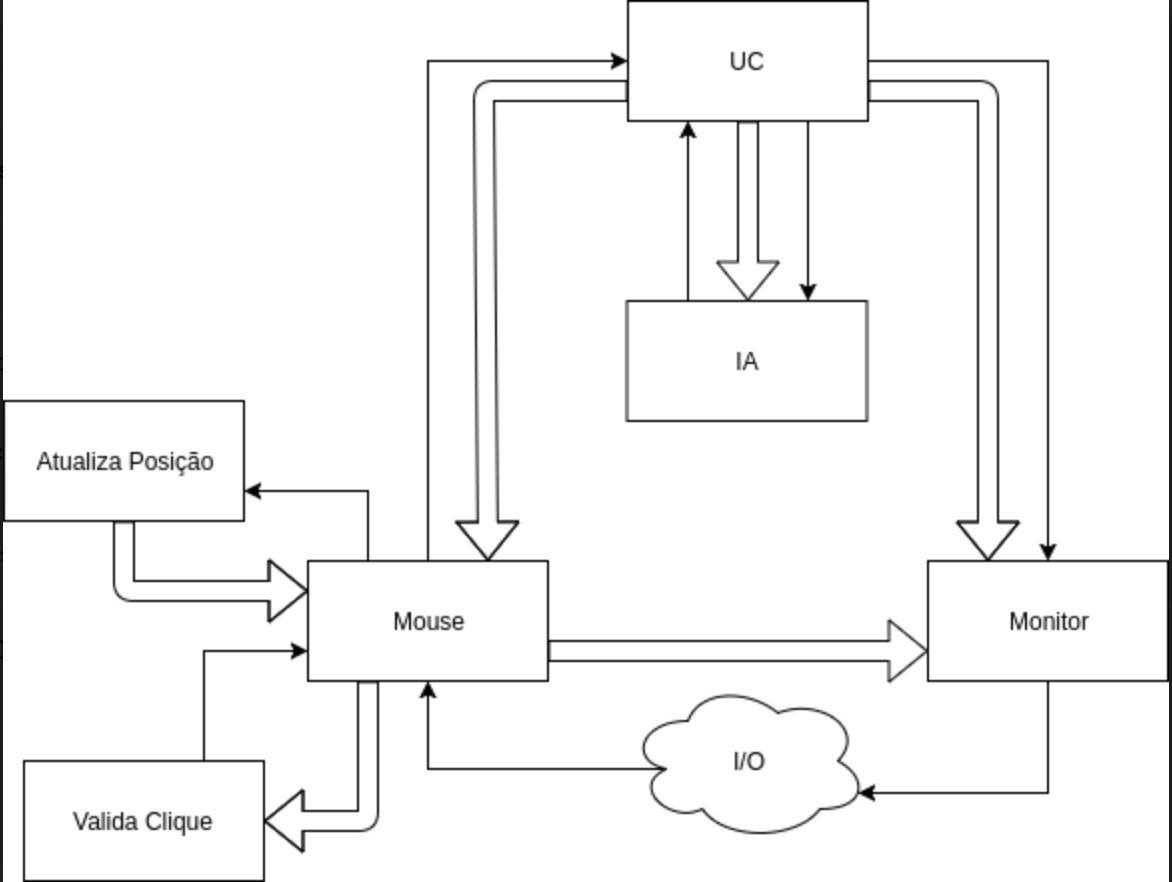
\includegraphics[height=8.2cm]{imagens/diagrama.png}
\caption{Diagrama de Blocos do jogo da velha implementado na placa DE1}
\label{fig:diagrama}
\end{figure}
